\documentclass{article} % For LaTeX2e
\usepackage{nips15submit_e,times}
\usepackage{hyperref}
\usepackage{url}
\usepackage{graphicx}
%\documentstyle[nips14submit_09,times,art10]{article} % For LaTeX 2.09
\title{End to End Differentiable Kernel Regression for Multivariate Time Series Using Convolutional Neural Networks}

\author{
Narges \\
\AND
David
}

% The \author macro works with any number of authors. There are two commands
% used to separate the names and addresses of multiple authors: \And and \AND.
%
% Using \And between authors leaves it to \LaTeX{} to determine where to break
% the lines. Using \AND forces a linebreak at that point. So, if \LaTeX{}
% puts 3 of 4 authors names on the first line, and the last on the second
% line, try using \AND instead of \And before the third author name.

\newcommand{\fix}{\marginpar{FIX}}
\newcommand{\new}{\marginpar{NEW}}

\nipsfinalcopy % Uncomment for camera-ready version

\begin{document}

\maketitle
\begin{abstract}
-Rewrite- Nonparametric methods have relied on parametric kernels and cross validation to recover the kernel family and optimal parameters. This severely limits the power of these methods in kernel density estimation, regression, and any consequent tasks. In this paper, we provide a simple formulation of nonparametric regression based on convolution, which enables us to learn the kernel function and parameters directly from temporal data. We show how learning kernels improves the quality of density estimation and regression, compared to traditional cross validation within parametric families of kernels. Moreover, we show our method can easily extend to multivariate input with structural and temporal dependencies. We compare to deep Gaussian Processes, and temporal autoencoders, and bidirectional LSTM for imputing missing values in multivariate time series.
\end{abstract}

\section{Introduction}

rewrite- In several areas of data science and machine learning, tractability of computations has often been traded off with simplifying assumption on the dependencies and distribution of the random variables of the model.\cite{} \cite{} \cite{} \cite{} As the size of datasets are growing, these assumptions begin to hurt more than they help \cite{} \cite{} \cite{}. Kernel density estimation\cite{} is one of the methods which does not impose most of the simplifying assumptions on the distribution of the data\cite{}, and has been previously studied in the context of density estimation, regression, causal inference, conditional distribution modeling, among others. Nonparametric regression\cite{} in particular, is a general method for estimating any function, given samples from the true distribution and a kernel similarity function.

While the theory of kernel regression allows the use of any positive semi definite kernel, in practice, methods only cross-validate over a few well-known kernel functions such as Radial basis(Gaussian), Laplace, or other simple kernels, and fail to consider the entire space of legal kernels. Of course when one leaves this step to cross-validation nothing more is reasonable to expect. In this paper, we try to liberate the kernel regression method from searching within a set of pre-defined kernel families.

In particular, we focus on irregularly measured temporal time series, and show how to construct a differentiable formulation of kernel density estimation for single time series as well as multiple dependent time series. Unlike most other multivariate models, our method can handle asynchronous observations of different variables across time. Our method is limited to discrete time observation, and we use a differentiable formalization and gradient descent to estimate the kernel function over its domain. As we show, not only this method is easily able to recover multivariate kernels, it also runs efficiently on large datasets.  

This paper is motivated by medical domain, where measurements of different biomarkers in our bodies are often performed asynchronously and measurements are often sparse in time. Models which impute the unobserved values between measurements can help discover abnormal temporal patterns and diagnose unknown diseases before late stage symptoms develop. We evaluate our method on a public temporal dataset (physionet challenge) and use the 

\section{Univatiate kernel regression: Learning the Kernel}
Imagine the input to be samples from D time series, each sampled irregularly. An example context would be different types of lab measurements for a patient at different time points across their life. We denote the samples as ${x^1_{t^1_1}}$, ${x^1_{t^1_2}}$, ..., ${x^1_{t^1_{n_1}}}$, ...,${x^D_{t^D_1}}$, ${x^D_{t^D_2}}$, ..., ${x^D_{t^D_{n_D}}}$, where $x^d$ refers to time series $d$ and $t^d_1$,... $t^d_{n_d}$ refer to the time points over which time series $d$ is sampled. 

Kernel regression provides a general formalism for estimating any function with additive noise. Let's start from a single time series, $x(t)$. Kernel regression assumes the following.

$$ x = f(t) + \epsilon $$
$$\epsilon \sim N(0,\sigma^2)$$

Given observed samples $x_{t_1}$,...$x_{t_n}$ from the series, general function regression with additive noise lets us estimate the value of $x$ at a new time point $t_{new}$ as follows. 

$$x(t_{new}) = \mathbf{E}_{x \sim P(x|t=t_{new})}[x] $$
$$\mathbf{E}_{x \sim P(x|t=t_{new})}[x] = \int_x x P(x|t=t_{new}) dx =\int_x x \frac{P(x , t=t_{new})}{P(t_{new})} dx $$

At this point, one can use kernel density estimation to estimate the probabilities $P(x , t=t_{new})$ and $P(t_{new})$ from the training data. Nadaraya\cite{} and Watson\cite{}showed that using a positive semidefinite kernel function $K(t, t')$, the nonparametric regression formulation is reduced to:

\begin{equation}
\mathbf{E}_{x \sim P(x|t=t_{new})}[x] = \frac{\sum_{i=1}^n{x_{t_{i}}K(t_{new}, t_{i})}} {\sum_{i=1}^n{K(t_{new}, t_{i})}}
\end{equation}

We can now rewrite the nonparametric regression using convolution operator. To be able to use functional notation, we first write the sequence of observed samples {$x_{t_1}$,...,$x_{t_n}$} as a function: $\bar X_{train}(t)$ = $\sum_{i=1}^{n} x_{t_i}\delta(t,{t_i})$, where $\delta(t,\tau_0) = 1$ when $t=\tau_0$, and 0 otherwise. 

Denoting convolution operator as $\ast$, i.e. $(k \ast f)(t) = \int_\tau K(t-\tau) f(\tau) d\tau$, the numerator of the kernel regression is equal to the following.

$$ \sum_{i=1}^n{x_{t_{i}}K(t_{i} - t_{new})} = (K \ast \bar X_{train}) (t_{new})$$

The denominator $P(t_{new})$ can similarly be written as a convolution of the kernel function with a sequence of $1$s at each point at which we have a sample, denoted as $I(\bar X_{train}:observed)(t) = \sum_{i=1}^{n}\delta(t,{t_i})$.

$$ \sum_{i=1}^n{K(t_{new}, t_{i})} = (K \ast I(\bar X_{train}:observed)) (t_{new}) $$

So the kernel regression formulation of Nadaraya and Watson reduces to the following formulation.

$$ \mathbf{E}_{x \sim P(x|t=t_{new})}[x] = \frac{(K \ast \bar X_{train}) (t_{new})}{(K \ast I(\bar X_{train} :observed)) (t_{new})} $$

This formulation has already been used in image processing literature\cite[] and \cite[], although with parametric kernels.  The benefit of this formulation is that we have a differentiable formulation of the kernel regression. Therefore we can learn $K(\tau)$ at each position $\tau$ within the kernel domain, using function composition and back-propagation\cite{}. We can also compose this differentiable kernel regression module within any subsequent differentiable operators and perform multiple tasks. In this paper we use leave-one-out imputation mean squared error as the loss function. In practice, we assume the domain of $K$ is bounded between $[-M, M]$, therefore the learning task will have $2M+1$ parameters.

Figure \ref{fig:arch} shows the architecture of this model.
% Figure \ref{fig:formulation} visually shows the process.
% \begin{figure}[h]
% \begin{center}
% 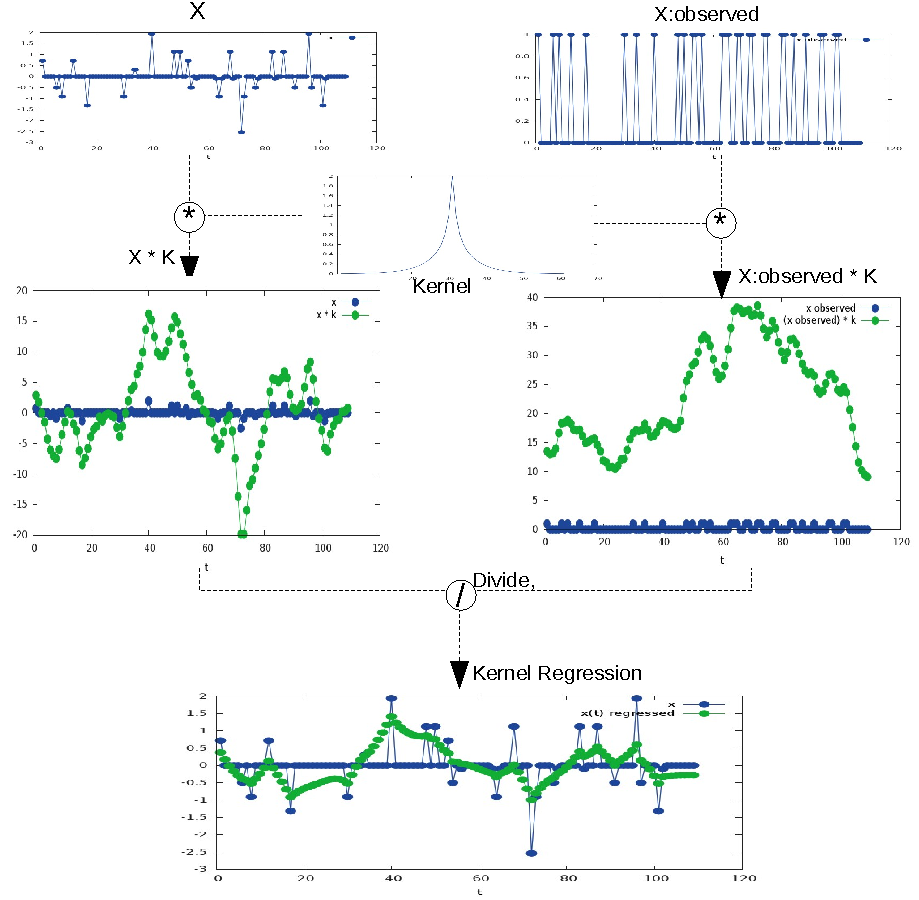
\includegraphics[width=15cm]{img/formulation-crop.pdf}
% \end{center}
% \caption{-redo- too big- Visualization of an example data series and kernel regression as convolution.}\label{fig:formulation}
% \end{figure}

\begin{figure}[h]
\begin{center}
\includegraphics[width=10cm]{img/univar-crop.pdf}
\end{center}
\caption{redo- too big - Architecture for kernel regression.}\label{fig:arch}
\end{figure}

\section{Multivariate kernel regression: Learning the temporal Kernel and Dependency structure}

Let's assume that we have $D$ time series now, where time series are sampled assynchronously. Traditional multivatiate kernel methods can not handle this case, because the kernels are defined over observations of all variables at each time point. Additionally, most traditional kernel methods assume the kernel to be the product of independent kernels on each dimension therefore missing the correlation structure between variables.

We provide two extensions of our univariate formulation of kernel regression here, also shown in figure \ref{fig:deepkr}. 

\subsection{Shallow Model: Linear Multivatiate Kernel}
In our first extension, we can extend the kernel $K$ to a matrix of size $D \times (2M+1)$, and optimize each kernel value between series $i$ at time $r$ and series $j$ at time $s$. The formulation of the kernel regression then becomes a 2D convolution of this kernel matrix with all time series' observed points in the numerator, normalized by the 2D convolution of the kernel matrix with a binary matrix encoding which series at which time point does have a nonzero observation. 

$$ \mathbf{E}_{x^d \sim P(x^d|t=t_{new})}[x^d] = \frac{(K \ast \bar X^{1..d}_{train})(t_{new})}{(K \ast I(\bar X^{1..d}_{train} :observed)) (t_{new})} $$

This formulation allows every variable at time t to be a linear function of all other variables between $t-M$ and $t+M$. An example shown in the experiments section includes a lab value that is a ratio of two other lab values by definition. If we hadn't known this in advance and applied multivariate kernel regression, based on this formualtion, the lab value is approximated with the difference of the two observations instead of the ratio. In practice, however, for many settings this formulation is sufficient and has strong empirical performance as we will show in experiments section.

\subsection{Deep Model: Nonlinear Multivatiate Kernel}

Our next extension involves a hierarchical structure shown in figure \ref{fig:deepkr} on the right. 
In the first layer we perform univariate kernel regression on each variable, and on the next layers we learn a general function that combines the intermediate 


\begin{figure}[h]
\begin{center}
\includegraphics[width=15cm]{img/deeparch-crop.pdf}
\end{center}
\caption{Architecture for Multivariate kernel regression.}\label{fig:deepkr}
\end{figure}

\section{Related Work}
traditional kernel methods, GP, univariat2e and multivariate.
(For GP)
http://www.cs.toronto.edu/~rgrosse/icml2013-gp.pdf
code: https://github.com/jamesrobertlloyd/gp-structure-search

\Section{Convoutional Neural Netowrks on Graphs with Unknown Structure}


\section{Experiments and Results}
\subsection{Data}
We normalize each series to be zero mean, unit variance (each measurement per person normalized on its own).. more details later..
Training data is 5K, and validation set is another 5K. There are 100 lab measurements over 109 months. 

\subsection{Synthetic Data}
Sampling multiple codependent Gaussian processe (I know how to do it)
How about other forms of dependencies??

\subsection{Data Augmentation for Training}
In order to successfully train the model with finite training data, we augmented each time series by adding Gaussian noise to each observation, and wiggling the time of each observation by a small amount, randomly drawn from another Gaussian distribution with standard deviation of 1. This step is very important for convergence of the method. 

\subsection{Technical Details of the implementation}
In order for the back-propagation to remain stable, we limited the derivative of the ratio such that if the magnitude of denominator was smaller than an epsilon, we did not back-propagate its derivative. We also filtered the gradients within range of [-10 +10], as higher values would potentially cause numerical instability. The effect of the limit was that the convergence would be slower, but more stable.


% \begin{table}[t]
% \caption{Sample table title}
% \label{sample-table}
% \begin{center}
% \begin{tabular}{ll}
% \multicolumn{1}{c}{\bf PART}  &\multicolumn{1}{c}{\bf DESCRIPTION}
% \\ \hline \\
% Dendrite         &Input terminal \\
% Axon             &Output terminal \\
% Soma             &Cell body (contains cell nucleus) \\
% \end{tabular}
% \end{center}
% \end{table}


\section{References}

\end{document}
